% !TeX root = ../main.tex
% Add the above to each chapter to make compiling the PDF easier in some editors.

\chapter{Offline Algorithms}\label{chapter:offline_algorithms}

To later measure the performance of online algorithms, we must first describe efficient offline algorithms that can be used to find optimal (or nearly optimal) solutions. In this chapter, we, therefore, describe algorithms for fractional and integral smoothed convex optimization. We begin with a general investigation of (fractional) convex optimization. Then, we turn to specific algorithms described in the literature for the uni-dimensional and multi-dimensional settings.

In our general argument, we want to use that the cost function $c_{\text{SCO}}$ is convex on $\mathcal{X}^T$ implying that algorithms for convex optimization can be used to solve the fractional offline case optimally.

\begin{lemma}
$c_{\text{SCO}}(X) = \sum_{t=1}^T f_t(X_t) + \norm{X_t - X_{t-1}}$ is convex on $\mathcal{X}^T$.
\end{lemma}
\begin{proof}
By definition $f_t$ is convex on $\mathcal{X}$. Every norm $\norm{\cdot}$ on $\mathcal{X}$ is convex by the triangle inequality as shown by the following argument: \begin{align*}
    \forall x, y \in \mathcal{X}.\ \forall \lambda \in [0,1].\ \norm{\lambda x + (1 - \lambda) y} \leq \norm{\lambda x} + \norm{(1 - \lambda) y} = \lambda \norm{x} + (1 - \lambda) \norm{y}.
\end{align*} In total we get that the sum of convex functions is also convex.
\end{proof}

\section{Convex Optimization}\label{section:offline_algorithms:convex_optimization}

As the offline variant of SCO simply is the problem of minimizing $c_{\text{SCO}}$, it is easy to see that we can use a convex optimization solver to obtain the optimal schedule $\hat{X}$. Throughout our discussion of algorithms, we denote schedules by $X$ and optimal solutions by $\hat{\cdot}$. Further, as we do not impose any constraints beyond the bounds of the decision space $\mathcal{X} \subset \mathbb{R}^d$ it suffices to find the local optimum of $c_{\text{SCO}}$ with respect to $\mathcal{X}$. By the convexity of $c_{\text{SCO}}$ we know that any local optimum will also be a global optimum~\cite{Bubeck2015}. We can choose the algorithm for finding the local optimum based on our knowledge of the properties of $c_{\text{SCO}}$. If, for example, $c_{\text{SCO}}$ is differentiable on $\mathcal{X}$ we could use gradient descent. In general, even if we cannot be sure of the differentiability of $c_{\text{SCO}}$ we can always find a subgradient in the interior of $\mathcal{X}$~\cite{Bubeck2015}. We denote by $\partial c_{\text{SCO}}(x)$ the set of subgradients of $c_{SCO}$ at the point $x \in \mathcal{X}$.

We are interested in finding good approximations of $\hat{x}$. To that end, we call a solution $\hat{x}$ \emph{$\epsilon$-optimal}\index{$\epsilon$-optimal solution} if $\norm{g(\hat{x})}^2 \leq \epsilon$ where $g \in \partial c_{\text{SCO}}(\hat{x})$. Using the projected subgradient method we are able to find an $\epsilon$-optimal solution $\hat{x}$ in $\mathcal{O}(1 / \epsilon^2)$ iterations~\cite{Boyd2003}. Note that this convergence rate is dimension-independent.

In our implementation, we use two different algorithms for derivative-free local optimization. We use the Subplex method, which extends the Nelder-Mead method if there are no equality or inequality constraints beyond the bounds on the decision space~\cite{Rowan1990}. If we impose such constraints, we use the COBYLA (Constrained Optimization BY Linear Approximations) algorithm, which iteratively constructs linear approximations of the objective functions and approximates constraints using a simplex in $d+1$ dimensions~\cite{Powell1994, Powell1998}. We use implementations from the NLopt library~\cite{Johnson}.

To be able to solve the optimization problem efficiently, it is crucial to quickly find a point $x \in \mathcal{X}$ of which the associated cost is finite. Until such a point is found, the algorithms sample values from the decision space without direction. Our primary use of convex optimization solvers is to determine a minimizer of the hitting cost. Furthermore, in the application of dynamically right-sizing data centers, hitting costs are always finite for the upper bound of the decision space. We, therefore, use this upper bound as the first guess for finding the minimizer even if this guess may be farther away from the minimizer than the lower bound. A convex optimization that does not terminate thus indicates that the problem is infeasible, for example, because the provided load profile is infeasible.

Note that we cannot draw this conclusion if we solve for a different objective, such as \cref{eq:heterogeneous_load_balancing_convex_program} or \cref{eq:multiple_load_types_load_balancing_convex_program}. In these cases, there is no guarantee that the solver will find a feasible point unless it searches over the entire decision space. In the given example, however, choosing the uniform distribution across all active server types performs well in practice. This heuristic ensures that no server type without at least one active server is assigned load, which would incur an infinite cost by definition.

We have seen a general method of solving high-dimensional (fractional) SCO, though the convergence rate could be increased using an accelerated gradient method if the hitting costs are strongly convex or conditional gradient descent if the hitting costs are smooth~\cite{Bubeck2015}. Denoting the complexity of computing the hitting cost $f_t$ by $\mathcal{O}(C)$ and the convergence rate of a convex optimization with $\alpha$ dimensions by $\mathcal{O}(O_{\epsilon}^{\alpha})$ we obtain a total complexity of $\mathcal{O}(T C O_{\epsilon}^{T d})$. We observe, however, that our method does not extend to the integral case, which is of particular importance for the application of right-sizing data centers. We, therefore, devote much of the remaining chapter to the discussion of algorithms for integral variants of SCO.

\section{Uni-Dimensional}

We now limit our attention to the uni-dimensional setting, i.e. $\mathcal{X} \subset \mathbb{R}$.

\subsection{Backward-Recurrent Capacity Provisioning}\label{section:offline_algorithms:ud:capacity_provisioning}

Before discussing algorithms for Int-SSCO, we discuss a simple backward-recurrent algorithm for SSCO proposed by \citeauthor{Lin2011}~\cite{Lin2011} based on capacity provisioning. They extend this idea to formulate an online algorithm which we discuss in \cref{section:online_algorithms:ud:lazy_capacity_provisioning}.

\citeauthor{Lin2011}~\cite{Lin2011} observed that the optimal offline solution can be characterized by two bounds corresponding to charging the switching cost for powering-up and powering-down servers, respectively. Let $\tau \in [T]$ be a time slot. Then the optimal offline solution $\hat{X}_{\tau}$ during time slot $\tau$ is lower bounded by $X_{\tau,\tau}^L$ where $X_{\tau}^L$ is the smallest vector minimizing \begin{align}\label{eq:ud:brcp:lower}
    c_{\tau}^L(X) = \sum_{t=1}^{\tau} f_t(X_t) + \beta (X_t - X_{t-1})^+.
\end{align} Conversely, $\hat{X}_{\tau}$ is upper bounded by $X_{\tau,\tau}^U$ where $X_{\tau}^U$ is the largest vector minimizing \begin{align}\label{eq:ud:brcp:upper}
    c_{\tau}^U(X) = \sum_{t=1}^{\tau} f_t(X_t) + \beta (X_{t-1} - X_t)^+.
\end{align} Overall we have $X_{\tau,\tau}^L \leq \hat{X}_{\tau} \leq X_{\tau,\tau}^U$~\cite{Lin2011}. Note that the switching cost is paid for powering up a server for the lower bound, while for the upper bound, the switching cost is paid for powering down a server. Further, it is easy to see that the bounds for time slot $\tau$ do not depend on any time slots $t > \tau$.

An optimal offline algorithm can be described as determining the optimal schedule moving backward in time. We begin by setting $\hat{X}_{T+1} = 0$. For each previous time slot $\tau$, we set $\hat{X}_{\tau} = \hat{X}_{\tau + 1}$ unless this violates the bounds, in which case we make the smallest possible change: \begin{align*}
    \hat{X}_{\tau} = \begin{cases}
        0 & \tau > T \\
        (\hat{X}_{\tau+1})_{X_{\tau,\tau}^L}^{X_{\tau,\tau}^U} & \tau \leq T
    \end{cases}
\end{align*} where $(\hat{X}_{\tau+1})_{X_{\tau,\tau}^L}^{X_{\tau,\tau}^U}$ is the projection of $\hat{X}_{\tau+1}$ onto $[X_{\tau,\tau}^L, X_{\tau,\tau}^U]$~\cite{Lin2011}. The resulting algorithm is described in \cref{alg:brcp}. We can use algorithms for convex optimization to compute the upper and lower bounds. Hence, we obtain a complexity of $\mathcal{O}(T^2 C O_{\epsilon}^T)$ for $\epsilon$-optimal upper and lower bounds. An example of Backward-Recurrent Capacity Provisioning is given in \cref{fig:backward_recurrent_capacity_provisioing_vs_lazy_capacity_provisioning}.

\begin{algorithm}
    \caption{Backward-Recurrent Capacity Provisioning~\cite{Lin2011}}\label{alg:brcp}
    \SetKwInOut{Input}{Input}
    \Input{$\mathcal{I}_{\text{SSCO}} = (T \in \mathbb{N}, m \in \mathbb{N}, \beta \in \mathbb{R}_{>0}, (f_1, \dots, f_T) \in (\mathbb{R}_{\geq 0} \to \mathbb{R}_{\geq 0})^T)$}
    $\hat{X}_{T+1} \gets 0$\;
    \For{$\tau \gets T$ \KwTo $1$}{
        find $X_{\tau,\tau}^L$ using the optimization described by \cref{eq:ud:brcp:lower}\;
        find $X_{\tau,\tau}^U$ using the optimization described by \cref{eq:ud:brcp:upper}\;
        $\hat{X}_{\tau} \gets (\hat{X}_{\tau+1})_{X_{\tau,\tau}^L}^{X_{\tau,\tau}^U}$\;
    }
    \Return $\hat{X}$\;
\end{algorithm}

\subsection{Graph-Based Optimal Integral Algorithm}\label{section:offline_algorithms:ud:graph_based}

We now turn to the uni-dimensional integral case of simplified smoothed convex optimization, i.e., our decision space is given as $\mathcal{X} := [m]_0$ where $m \in \mathbb{N}$ is the maximum number of servers a data center can employ at the same time. As our decision space is discrete and finite, it is natural to model our problem as a weighted directed graph which is comprised of vertices $v_{t,j}$ for each $t \in [T]$ and $j \in [m]_0$ describing the state that during time slot $t$ exactly $j$ servers are active. For the initial and final state $X_0 = X_{T+1} = 0$ we have two additional vertices $v_{0,0}$ and $v_{T+1,0}$. For each vertice associated with time slot $t \in [T]_0$ we add an edge to all vertices associated with the subsequent time slot $t + 1$. With each edge from $v_{t,i}$ to $v_{t+1,j}$ we associate the switching cost incurred by the represented action, i.e. $\beta (j - i)^+$, and the hitting cost incurred by the state represented by the vertice $v_{t+1,j}$, i.e. $f_{t+1}(j)$. The structure of this graph is presented in \cref{fig:underlying_graph_of_uni_dimensional_integral_offline_algorithm}.

\begin{figure}
    \centering
    \resizebox{\textwidth}{!}{

\tikzset{every picture/.style={line width=0.75pt}} %set default line width to 0.75pt        

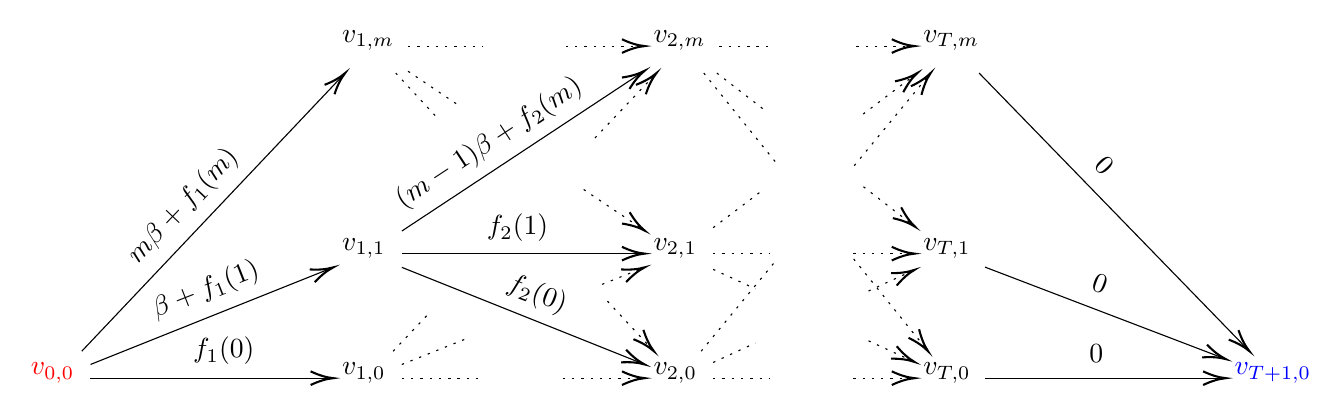
\begin{tikzpicture}[x=0.75pt,y=0.75pt,yscale=-1,xscale=1]
%uncomment if require: \path (0,428); %set diagram left start at 0, and has height of 428


% Text Node
\draw (59,252.4) node [anchor=north west][inner sep=0.75pt]  [color={rgb, 255:red, 255; green, 0; blue, 0 }  ,opacity=1 ]  {$v_{0,0}$};
% Text Node
\draw (209,252.4) node [anchor=north west][inner sep=0.75pt]    {$v_{1,0}$};
% Text Node
\draw (209,192.4) node [anchor=north west][inner sep=0.75pt]    {$v_{1,1}$};
% Text Node
\draw (209,92.4) node [anchor=north west][inner sep=0.75pt]    {$v_{1,m}$};
% Text Node
\draw (359,252.4) node [anchor=north west][inner sep=0.75pt]    {$v_{2,0}$};
% Text Node
\draw (359,192.4) node [anchor=north west][inner sep=0.75pt]    {$v_{2,1}$};
% Text Node
\draw (359,92.4) node [anchor=north west][inner sep=0.75pt]    {$v_{2,m}$};
% Text Node
\draw (489,252.4) node [anchor=north west][inner sep=0.75pt]    {$v_{T,0}$};
% Text Node
\draw (489,192.4) node [anchor=north west][inner sep=0.75pt]    {$v_{T,1}$};
% Text Node
\draw (489,92.4) node [anchor=north west][inner sep=0.75pt]    {$v_{T,m}$};
% Text Node
\draw (639,252.4) node [anchor=north west][inner sep=0.75pt]  [color={rgb, 255:red, 0; green, 0; blue, 255 }  ,opacity=1 ]  {$v_{T+1,0}$};
% Text Node
\draw (425,94.4) node [anchor=north west][inner sep=0.75pt]    {$\dotsc $};
% Text Node
\draw (425,194.4) node [anchor=north west][inner sep=0.75pt]    {$\dotsc $};
% Text Node
\draw (425,254.4) node [anchor=north west][inner sep=0.75pt]    {$\dotsc $};
% Text Node
\draw (578.43,151.42) node [anchor=north west][inner sep=0.75pt]  [rotate=-46.76]  {$0$};
% Text Node
\draw (573.07,208.77) node [anchor=north west][inner sep=0.75pt]  [rotate=-20.66]  {$0$};
% Text Node
\draw (569,243.4) node [anchor=north west][inner sep=0.75pt]    {$0$};
% Text Node
\draw (102.7,199.18) node [anchor=north west][inner sep=0.75pt]  [rotate=-313.5]  {$m\beta +f_{1}( m)$};
% Text Node
\draw (115.31,221.53) node [anchor=north west][inner sep=0.75pt]  [rotate=-338.49]  {$\beta +f_{1}( 1)$};
% Text Node
\draw (137.2,240.01) node [anchor=north west][inner sep=0.75pt]    {$f_{1}( 0)$};
% Text Node
\draw (232.09,170.58) node [anchor=north west][inner sep=0.75pt]  [rotate=-326.72]  {$( m-1) \beta +f_{2}( m)$};
% Text Node
\draw (278.69,180.75) node [anchor=north west][inner sep=0.75pt]    {$f_{2}( 1)$};
% Text Node
\draw (292.03,207.51) node [anchor=north west][inner sep=0.75pt]  [rotate=-21]  {$f_{2}( 0)$};
% Connection
\draw    (89,261) -- (204,261) ;
\draw [shift={(206,261)}, rotate = 180] [color={rgb, 255:red, 0; green, 0; blue, 0 }  ][line width=0.75]    (10.93,-3.29) .. controls (6.95,-1.4) and (3.31,-0.3) .. (0,0) .. controls (3.31,0.3) and (6.95,1.4) .. (10.93,3.29)   ;
% Connection
\draw    (89,254.4) -- (204.14,208.34) ;
\draw [shift={(206,207.6)}, rotate = 518.2] [color={rgb, 255:red, 0; green, 0; blue, 0 }  ][line width=0.75]    (10.93,-3.29) .. controls (6.95,-1.4) and (3.31,-0.3) .. (0,0) .. controls (3.31,0.3) and (6.95,1.4) .. (10.93,3.29)   ;
% Connection
\draw    (84.81,248) -- (210.32,115.45) ;
\draw [shift={(211.69,114)}, rotate = 493.44] [color={rgb, 255:red, 0; green, 0; blue, 0 }  ][line width=0.75]    (10.93,-3.29) .. controls (6.95,-1.4) and (3.31,-0.3) .. (0,0) .. controls (3.31,0.3) and (6.95,1.4) .. (10.93,3.29)   ;
% Connection
\draw  [dash pattern={on 0.84pt off 2.51pt}]  (242,101) -- (278,101)(318,101) -- (354,101) ;
\draw [shift={(356,101)}, rotate = 180] [color={rgb, 255:red, 0; green, 0; blue, 0 }  ][line width=0.75]    (10.93,-3.29) .. controls (6.95,-1.4) and (3.31,-0.3) .. (0,0) .. controls (3.31,0.3) and (6.95,1.4) .. (10.93,3.29)   ;
% Connection
\draw  [dash pattern={on 0.84pt off 2.51pt}]  (242,113.12) -- (265.23,128.77)(326.61,170.1) -- (354.34,188.77) ;
\draw [shift={(356,189.89)}, rotate = 213.96] [color={rgb, 255:red, 0; green, 0; blue, 0 }  ][line width=0.75]    (10.93,-3.29) .. controls (6.95,-1.4) and (3.31,-0.3) .. (0,0) .. controls (3.31,0.3) and (6.95,1.4) .. (10.93,3.29)   ;
% Connection
\draw  [dash pattern={on 0.84pt off 2.51pt}]  (236.07,114) -- (257.09,136.66)(338.05,223.88) -- (359.07,246.53) ;
\draw [shift={(360.43,248)}, rotate = 227.13] [color={rgb, 255:red, 0; green, 0; blue, 0 }  ][line width=0.75]    (10.93,-3.29) .. controls (6.95,-1.4) and (3.31,-0.3) .. (0,0) .. controls (3.31,0.3) and (6.95,1.4) .. (10.93,3.29)   ;
% Connection
\draw  [dash pattern={on 0.84pt off 2.51pt}]  (239,261) -- (276.5,261)(316.5,261) -- (354,261) ;
\draw [shift={(356,261)}, rotate = 180] [color={rgb, 255:red, 0; green, 0; blue, 0 }  ][line width=0.75]    (10.93,-3.29) .. controls (6.95,-1.4) and (3.31,-0.3) .. (0,0) .. controls (3.31,0.3) and (6.95,1.4) .. (10.93,3.29)   ;
% Connection
\draw  [dash pattern={on 0.84pt off 2.51pt}]  (239,254.4) -- (271.45,241.42)(335.52,215.79) -- (354.14,208.34) ;
\draw [shift={(356,207.6)}, rotate = 518.2] [color={rgb, 255:red, 0; green, 0; blue, 0 }  ][line width=0.75]    (10.93,-3.29) .. controls (6.95,-1.4) and (3.31,-0.3) .. (0,0) .. controls (3.31,0.3) and (6.95,1.4) .. (10.93,3.29)   ;
% Connection
\draw  [dash pattern={on 0.84pt off 2.51pt}]  (234.81,248) -- (253.01,228.78)(332.08,145.27) -- (360.32,115.45) ;
\draw [shift={(361.69,114)}, rotate = 493.44] [color={rgb, 255:red, 0; green, 0; blue, 0 }  ][line width=0.75]    (10.93,-3.29) .. controls (6.95,-1.4) and (3.31,-0.3) .. (0,0) .. controls (3.31,0.3) and (6.95,1.4) .. (10.93,3.29)   ;
% Connection
\draw    (239,207.6) -- (354.14,253.66) ;
\draw [shift={(356,254.4)}, rotate = 201.8] [color={rgb, 255:red, 0; green, 0; blue, 0 }  ][line width=0.75]    (10.93,-3.29) .. controls (6.95,-1.4) and (3.31,-0.3) .. (0,0) .. controls (3.31,0.3) and (6.95,1.4) .. (10.93,3.29)   ;
% Connection
\draw    (239,201) -- (354,201) ;
\draw [shift={(356,201)}, rotate = 180] [color={rgb, 255:red, 0; green, 0; blue, 0 }  ][line width=0.75]    (10.93,-3.29) .. controls (6.95,-1.4) and (3.31,-0.3) .. (0,0) .. controls (3.31,0.3) and (6.95,1.4) .. (10.93,3.29)   ;
% Connection
\draw    (239,190.11) -- (354.33,113.98) ;
\draw [shift={(356,112.88)}, rotate = 506.57] [color={rgb, 255:red, 0; green, 0; blue, 0 }  ][line width=0.75]    (10.93,-3.29) .. controls (6.95,-1.4) and (3.31,-0.3) .. (0,0) .. controls (3.31,0.3) and (6.95,1.4) .. (10.93,3.29)   ;
% Connection
\draw  [dash pattern={on 0.84pt off 2.51pt}]  (392,101) -- (418,101)(458,101) -- (484,101) ;
\draw [shift={(486,101)}, rotate = 180] [color={rgb, 255:red, 0; green, 0; blue, 0 }  ][line width=0.75]    (10.93,-3.29) .. controls (6.95,-1.4) and (3.31,-0.3) .. (0,0) .. controls (3.31,0.3) and (6.95,1.4) .. (10.93,3.29)   ;
% Connection
\draw  [dash pattern={on 0.84pt off 2.51pt}]  (390.77,114) -- (414,132.01)(461.42,168.77) -- (484.65,186.77) ;
\draw [shift={(486.23,188)}, rotate = 217.78] [color={rgb, 255:red, 0; green, 0; blue, 0 }  ][line width=0.75]    (10.93,-3.29) .. controls (6.95,-1.4) and (3.31,-0.3) .. (0,0) .. controls (3.31,0.3) and (6.95,1.4) .. (10.93,3.29)   ;
% Connection
\draw  [dash pattern={on 0.84pt off 2.51pt}]  (384.48,114) -- (419.04,156.86)(456.7,203.57) -- (491.26,246.44) ;
\draw [shift={(492.52,248)}, rotate = 231.12] [color={rgb, 255:red, 0; green, 0; blue, 0 }  ][line width=0.75]    (10.93,-3.29) .. controls (6.95,-1.4) and (3.31,-0.3) .. (0,0) .. controls (3.31,0.3) and (6.95,1.4) .. (10.93,3.29)   ;
% Connection
\draw  [dash pattern={on 0.84pt off 2.51pt}]  (389,261) -- (416.5,261)(456.5,261) -- (484,261) ;
\draw [shift={(486,261)}, rotate = 180] [color={rgb, 255:red, 0; green, 0; blue, 0 }  ][line width=0.75]    (10.93,-3.29) .. controls (6.95,-1.4) and (3.31,-0.3) .. (0,0) .. controls (3.31,0.3) and (6.95,1.4) .. (10.93,3.29)   ;
% Connection
\draw  [dash pattern={on 0.84pt off 2.51pt}]  (389,253.41) -- (409.33,244.06)(463.85,219) -- (484.18,209.65) ;
\draw [shift={(486,208.82)}, rotate = 515.31] [color={rgb, 255:red, 0; green, 0; blue, 0 }  ][line width=0.75]    (10.93,-3.29) .. controls (6.95,-1.4) and (3.31,-0.3) .. (0,0) .. controls (3.31,0.3) and (6.95,1.4) .. (10.93,3.29)   ;
% Connection
\draw  [dash pattern={on 0.84pt off 2.51pt}]  (383.23,248) -- (418.77,204.91)(456.96,158.63) -- (492.5,115.54) ;
\draw [shift={(493.78,114)}, rotate = 489.52] [color={rgb, 255:red, 0; green, 0; blue, 0 }  ][line width=0.75]    (10.93,-3.29) .. controls (6.95,-1.4) and (3.31,-0.3) .. (0,0) .. controls (3.31,0.3) and (6.95,1.4) .. (10.93,3.29)   ;
% Connection
\draw  [dash pattern={on 0.84pt off 2.51pt}]  (389,208.59) -- (409.33,217.94)(463.85,243) -- (484.18,252.35) ;
\draw [shift={(486,253.18)}, rotate = 204.69] [color={rgb, 255:red, 0; green, 0; blue, 0 }  ][line width=0.75]    (10.93,-3.29) .. controls (6.95,-1.4) and (3.31,-0.3) .. (0,0) .. controls (3.31,0.3) and (6.95,1.4) .. (10.93,3.29)   ;
% Connection
\draw  [dash pattern={on 0.84pt off 2.51pt}]  (389,201) -- (416.5,201)(456.5,201) -- (484,201) ;
\draw [shift={(486,201)}, rotate = 180] [color={rgb, 255:red, 0; green, 0; blue, 0 }  ][line width=0.75]    (10.93,-3.29) .. controls (6.95,-1.4) and (3.31,-0.3) .. (0,0) .. controls (3.31,0.3) and (6.95,1.4) .. (10.93,3.29)   ;
% Connection
\draw  [dash pattern={on 0.84pt off 2.51pt}]  (389,188.5) -- (413.46,169.97)(461.29,133.74) -- (485.75,115.21) ;
\draw [shift={(487.34,114)}, rotate = 502.85] [color={rgb, 255:red, 0; green, 0; blue, 0 }  ][line width=0.75]    (10.93,-3.29) .. controls (6.95,-1.4) and (3.31,-0.3) .. (0,0) .. controls (3.31,0.3) and (6.95,1.4) .. (10.93,3.29)   ;
% Connection
\draw    (520,261) -- (634,261) ;
\draw [shift={(636,261)}, rotate = 180] [color={rgb, 255:red, 0; green, 0; blue, 0 }  ][line width=0.75]    (10.93,-3.29) .. controls (6.95,-1.4) and (3.31,-0.3) .. (0,0) .. controls (3.31,0.3) and (6.95,1.4) .. (10.93,3.29)   ;
% Connection
\draw    (520,207.5) -- (634.13,251.11) ;
\draw [shift={(636,251.83)}, rotate = 200.92000000000002] [color={rgb, 255:red, 0; green, 0; blue, 0 }  ][line width=0.75]    (10.93,-3.29) .. controls (6.95,-1.4) and (3.31,-0.3) .. (0,0) .. controls (3.31,0.3) and (6.95,1.4) .. (10.93,3.29)   ;
% Connection
\draw    (517.13,114) -- (645.97,246.57) ;
\draw [shift={(647.37,248)}, rotate = 225.82] [color={rgb, 255:red, 0; green, 0; blue, 0 }  ][line width=0.75]    (10.93,-3.29) .. controls (6.95,-1.4) and (3.31,-0.3) .. (0,0) .. controls (3.31,0.3) and (6.95,1.4) .. (10.93,3.29)   ;

\end{tikzpicture}
}
    \caption{Underlying graph of uni-dimensional integral offline algorithm. The algorithm finds a shortest path from $v_{0,0}$ (red) to $v_{T+1,0}$ (blue).}
    \label{fig:underlying_graph_of_uni_dimensional_integral_offline_algorithm}
\end{figure}

\citeauthor{Albers2018}~\cite{Albers2018} show that an optimal schedule is given by the shortest path from $v_{0,0}$ to $v_{T+1,0}$ within our constructed graph. We observe that our graph follows a particular structure. Each vertice representing an action during time slot $t$ can only be reached by a path that includes precisely one vertice representing time slots $0$ through $t - 1$ and, crucially, whether this path is optimal up to time $t$ does not depend on any time slot past $t$. Bellman's principle of optimality states that any part of an optimal path must itself be optimal~\cite{Bellman1954}. Based on this principle and using our previous observation, we can use dynamic programming to sequentially determine the optimal paths to the vertices of time slot $t$.

Moreover, we observe a second property of the graph of interest. Namely, for each time slot $t \in [T]$ (in the following called columns), the graph has precisely $m$ vertices (in the following called rows), which can only be reached through edges from vertices representing time slot $t - 1$ and all outgoing edges lead to vertices representing time slot $t + 1$. We are, therefore, able to iteratively solve the problem of finding a shortest path for subgraphs of our original graph using binary search. During each iteration, we only consider a constant number of rows.

To simplify the selection of rows, the algorithm assumes $m$ to be a power of two. Instances $\mathcal{I} = (T, m, \beta, F)$ where $m$ is not a power of two can be transformed into an instance $\mathcal{I}' = (T, m', \beta, F')$ with $m' = 2^{\lceil \log_2 m \rceil}$, $F' = (f'_1, \dots f'_T)$, and \begin{align*}
    f'_t(x) = \begin{cases}
        f_t(x) & x \leq m \\
        x (f_t(m) + \epsilon) & \text{otherwise} \\
    \end{cases}
\end{align*} for $\epsilon > 0$. The algorithm using $\log_2 m - 1$ iterations is described in \cref{alg:ud:optimal_graph_search}. During each iteration the algorithm finds the shortest path in a subgraph comprised of only five rows in $\mathcal{O}(T C)$ time. Overall, we thus find an optimal schedule in $\mathcal{O}(T C \log_2 m)$ time. \citeauthor{Albers2018}~\cite{Albers2018} show that in the final iteration, the algorithm obtains an optimal schedule for the original problem instance.

\begin{algorithm}
    \caption{Uni-Dimensional Optimal Graph Search~\cite{Albers2018}}\label{alg:ud:optimal_graph_search}
    \KwIn{$\mathcal{I}_{\text{Int-SSCO}} = (T \in \mathbb{N}, m \in \mathbb{N}, \beta \in \mathbb{R}_{>0}, (f_1, \dots, f_T) \in ([m]_0 \to \mathbb{R}_{\geq 0})^T)$ with $m$ a power of two}
    \eIf{$m > 2$}{$K \gets \log_2 m - 2$ }{$K \gets 0$ }
    $V^K \gets \{v_{0,0}, v_{T+1,0}\} \cup \{v_{t,\xi m / 4} \mid t \in [T], \xi \in [4]_0\}$\;
    $\hat{X}^K \gets \text{\ref{proc:ud:optimal_graph_search:shortest_path}}(\mathcal{I}_{Int-SSCO}, V^K)$\;
    \For{$k \gets K - 1$ \KwTo $0$}{
        $V_t^k \gets \{\hat{X}_t^{k+1} + \xi 2^k \mid \xi \in \{-2, -1, 0, 1, 2\}\} \cap [m]_0$\;
        $V^k \gets \{v_{0,0}, v_{T+1,0}\} \cup \{v_{t,j} \mid t \in [T], j \in V_t^k\}$\;
        $\hat{X}^k \gets \text{\ref{proc:ud:optimal_graph_search:shortest_path}}(\mathcal{I}_{Int-SSCO}, V^k)$\;
    }
    \Return $\hat{X}^0$\;
\end{algorithm}

\begin{function}
	\caption{ShortestPath($\mathcal{I}, V$)}\label{proc:ud:optimal_graph_search:shortest_path}
	\For{$t \gets 1$ \KwTo $T$}{
        \ForEach{$v_{t,j} \in V$}{
            $\hat{c}^{v_{t,j}} \gets \infty$\;
            \ForEach{$v_{t-1,i} \in V$}{
                $c^{v_{t,j}} \gets \hat{c}^{v_{t-1,i}} + f_t(j) + \beta (j - i)^+$\;
                \If{$c^{v_{t,j}} < \hat{c}^{v_{t,j}}$}{
                    $\hat{c}^{v_{t,j}} \gets c^{v_{t,j}}$\;
                    $\hat{X}^{v_{t,j}} \gets \hat{X}^{v_{t-1,i}}$\;
                }
            }
            $\hat{X}_t^{v_{t,j}} \gets j$\;
        }
    }
    $\hat{v} \gets \argmin_{v_{T,j} \in V} \hat{c}^{v_{T,j}}$\;
	\Return $\hat{X}^{\hat{v}}$\;
\end{function}

\section{Multi-Dimensional}

\subsection{Graph-Based Optimal Integral Algorithm}

We now lift the restriction on $d$ and also consider multi-dimensional instances of Int-SSCO. Again, an intuitive approach is to model the offline problem using a graph. Previously, with $d = 1$, the vertices where arranged in a two-dimensional grid (time being the first dimension). We now arrange the vertices in a $(d+1)$-dimensional grid. We call $x = (x_1, \dots, x_d) \in \mathcal{M}$ a \emph{configuration}\index{configuration} (also called a state in the literature) where $M_k := [m_k]_0$ and $\mathcal{M} := M_1 \times \dots \times M_d = \mathcal{X}$ is the set of all configurations. For each configuration $x$ and each time slot $t$ we introduce two vertices. $v_{t,x}^{\uparrow}$ represents the configuration in the beginning of time slot $t$ while $v_{t,x}^{\downarrow}$ represents the configuration at the end of time slot $t$. Thus, the first dimension has $2 T$ \emph{layers} where each layer only consists of powering-up or powering-down vertices.

In our graph we have edges $e_{t,x,k}^{\uparrow}$ representing the powering-up of a server of type $k$ in the beginning of time slot $t$, edges $e_{t,x}^{\text{op}}$ representing operating configuration $x$ during time slot $t$, edges $e_{t,x,k}^{\downarrow}$ representing the powering-down of a server of type $k$ at the end of time slot $t$, and edges $e_{t,x}^{\rightarrow}$ transitioning to the next time slot. For each $k \in [d]$ and $x = (x_1, \dots, x_d) \in [m_1]_0 \times \dots \times [m_k - 1]_0 \times \dots \times [m_d]_0$ let $x' = (x_1, \dots, x_k + 1, \dots, x_d)$. We add an edge $e_{t,x,k}^{\uparrow}$ between $v_{t,x}^{\uparrow}$ and $v_{t,x'}^{\uparrow}$ with weight $\beta_k$ and another edge $e_{t,x,k}^{\downarrow}$ between $v_{t,x'}^{\downarrow}$ and $v_{t,x}^{\downarrow}$ with weight $0$. For each time slot $t \in [T]$ and $x \in \mathcal{M}$, we add the edge $e_{t,x}^{\text{op}}$ from $v_{t,x}^{\uparrow}$ to $v_{t,x}^{\downarrow}$ with weight $f_t(x)$. Lastly, for each $t \in [T-1]$ and $x \in \mathcal{M}$, we add the edge $e_{t,x}^{\rightarrow}$ from $v_{t,x}^{\downarrow}$ to $v_{t+1,x}^{\uparrow}$ with weight $0$.  To simplify the algorithm we add an additional vertice $v_{T+1,\mathbf{0}}^{\uparrow}$ which can be reached through the edge $e_{t,\mathbf{0}}^{\rightarrow}$ from $v_{t,\mathbf{0}}^{\downarrow}$. The structure of this graph is presented in \cref{fig:underlying_graph_of_the_multi_dimensional_integral_offline_algorithm}.

\begin{figure}
    \centering
    \resizebox{\textwidth}{!}{

\tikzset{every picture/.style={line width=0.75pt}} %set default line width to 0.75pt        

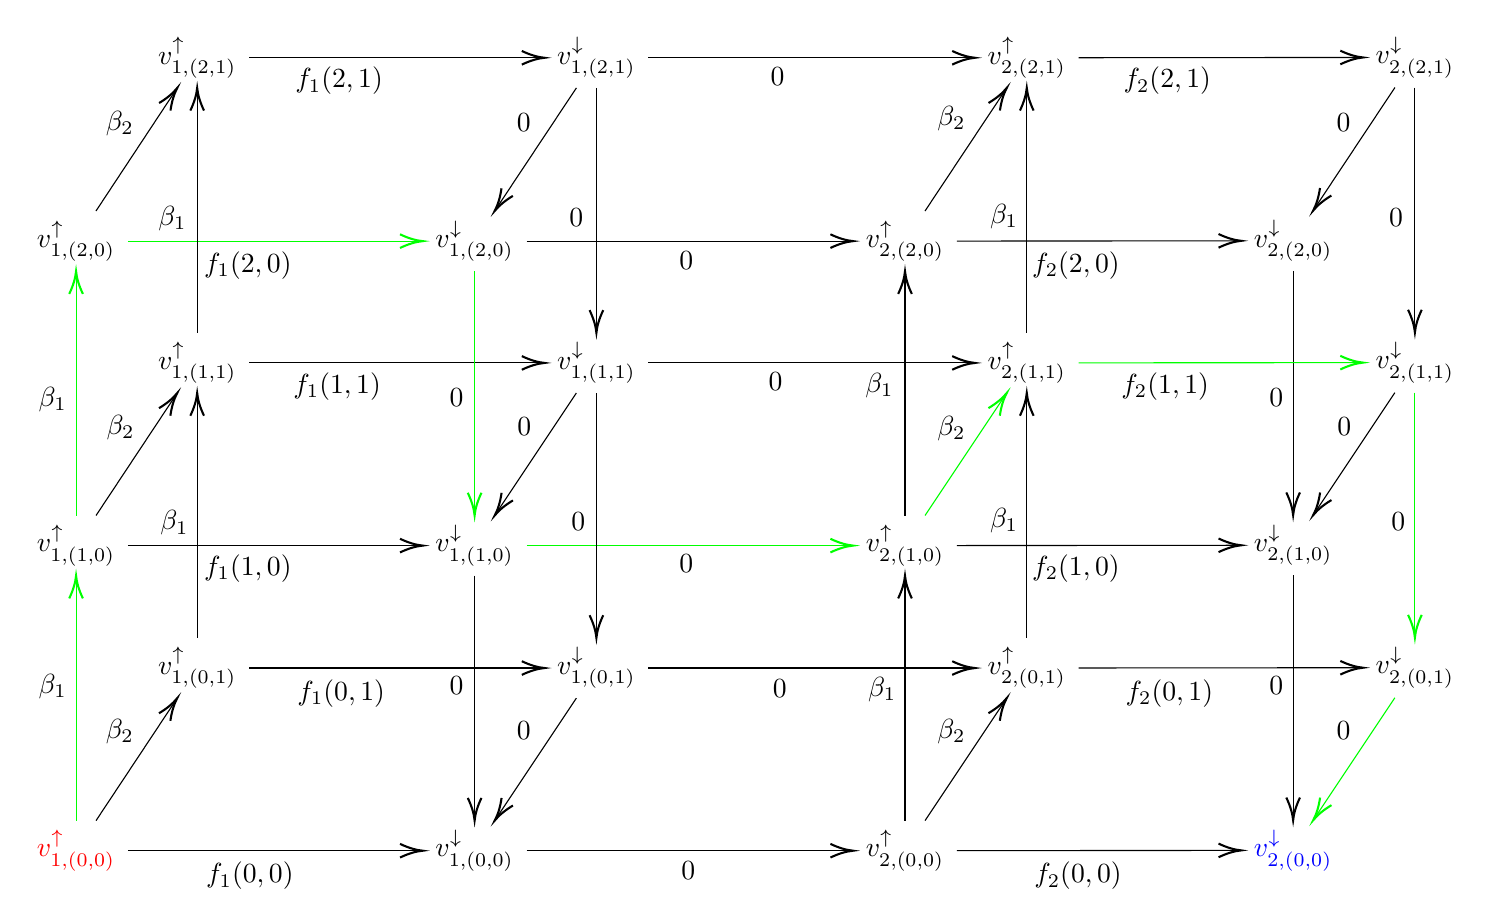
\begin{tikzpicture}[x=0.75pt,y=0.75pt,yscale=-1,xscale=1]
%uncomment if require: \path (0,428); %set diagram left start at 0, and has height of 428



% Text Node
\draw (28.6,115.48) node    {$v_{1,( 2,0)}^{\uparrow }$};
% Text Node
\draw (86.95,27.14) node    {$v_{1,( 2,1)}^{\uparrow }$};
% Text Node
\draw (28.6,262.17) node    {$v_{1,( 1,0)}^{\uparrow }$};
% Text Node
\draw (279.3,27.14) node    {$v_{1,( 2,1)}^{\downarrow }$};
% Text Node
\draw (486.65,27.14) node    {$v_{2,( 2,1)}^{\uparrow }$};
% Text Node
\draw (220.62,115.48) node    {$v_{1,( 2,0)}^{\downarrow }$};
% Text Node
\draw (427.98,115.48) node    {$v_{2,( 2,0)}^{\uparrow }$};
% Text Node
\draw (86.95,174.16) node    {$v_{1,( 1,1)}^{\uparrow }$};
% Text Node
\draw (279.3,174.16) node    {$v_{1,( 1,1)}^{\downarrow }$};
% Text Node
\draw (486.65,174.16) node    {$v_{2,( 1,1)}^{\uparrow }$};
% Text Node
\draw (220.62,262.17) node    {$v_{1,( 1,0)}^{\downarrow }$};
% Text Node
\draw (427.98,262.17) node    {$v_{2,( 1,0)}^{\uparrow }$};
% Text Node
\draw (673.65,26.96) node    {$v_{2,( 2,1)}^{\downarrow }$};
% Text Node
\draw (614.98,115.31) node    {$v_{2,( 2,0)}^{\downarrow }$};
% Text Node
\draw (673.65,173.99) node    {$v_{2,( 1,1)}^{\downarrow }$};
% Text Node
\draw (614.98,262) node    {$v_{2,( 1,0)}^{\downarrow }$};
% Text Node
\draw (28.6,409.17) node  [color={rgb, 255:red, 255; green, 0; blue, 0 }  ,opacity=1 ]  {$v_{1,( 0,0)}^{\uparrow }$};
% Text Node
\draw (86.95,321.16) node    {$v_{1,( 0,1)}^{\uparrow }$};
% Text Node
\draw (279.3,321.16) node    {$v_{1,( 0,1)}^{\downarrow }$};
% Text Node
\draw (486.65,321.16) node    {$v_{2,( 0,1)}^{\uparrow }$};
% Text Node
\draw (220.62,409.17) node    {$v_{1,( 0,0)}^{\downarrow }$};
% Text Node
\draw (427.98,409.17) node    {$v_{2,( 0,0)}^{\uparrow }$};
% Text Node
\draw (673.65,320.99) node    {$v_{2,( 0,1)}^{\downarrow }$};
% Text Node
\draw (614.98,409) node  [color={rgb, 255:red, 0; green, 0; blue, 255 }  ,opacity=1 ]  {$v_{2,( 0,0)}^{\downarrow }$};
% Text Node
\draw (9.33,323.07) node [anchor=north west][inner sep=0.75pt]    {$\beta _{1}$};
% Text Node
\draw (9.33,184.4) node [anchor=north west][inner sep=0.75pt]    {$\beta _{1}$};
% Text Node
\draw (41.67,51.73) node [anchor=north west][inner sep=0.75pt]    {$\beta _{2}$};
% Text Node
\draw (42,198.07) node [anchor=north west][inner sep=0.75pt]    {$\beta _{2}$};
% Text Node
\draw (41.67,344.73) node [anchor=north west][inner sep=0.75pt]    {$\beta _{2}$};
% Text Node
\draw (67,97.4) node [anchor=north west][inner sep=0.75pt]    {$\beta _{1}$};
% Text Node
\draw (68,244.07) node [anchor=north west][inner sep=0.75pt]    {$\beta _{1}$};
% Text Node
\draw (409,324.4) node [anchor=north west][inner sep=0.75pt]    {$\beta _{1}$};
% Text Node
\draw (407.67,177.73) node [anchor=north west][inner sep=0.75pt]    {$\beta _{1}$};
% Text Node
\draw (467.67,96.4) node [anchor=north west][inner sep=0.75pt]    {$\beta _{1}$};
% Text Node
\draw (467.67,243.07) node [anchor=north west][inner sep=0.75pt]    {$\beta _{1}$};
% Text Node
\draw (442.33,49.07) node [anchor=north west][inner sep=0.75pt]    {$\beta _{2}$};
% Text Node
\draw (442.33,198.4) node [anchor=north west][inner sep=0.75pt]    {$\beta _{2}$};
% Text Node
\draw (442.33,344.4) node [anchor=north west][inner sep=0.75pt]    {$\beta _{2}$};
% Text Node
\draw (207.33,324.07) node [anchor=north west][inner sep=0.75pt]    {$0$};
% Text Node
\draw (207.33,185.4) node [anchor=north west][inner sep=0.75pt]    {$0$};
% Text Node
\draw (239.67,52.73) node [anchor=north west][inner sep=0.75pt]    {$0$};
% Text Node
\draw (240,199.07) node [anchor=north west][inner sep=0.75pt]    {$0$};
% Text Node
\draw (239.67,345.73) node [anchor=north west][inner sep=0.75pt]    {$0$};
% Text Node
\draw (265,98.4) node [anchor=north west][inner sep=0.75pt]    {$0$};
% Text Node
\draw (266,245.07) node [anchor=north west][inner sep=0.75pt]    {$0$};
% Text Node
\draw (602.33,324.07) node [anchor=north west][inner sep=0.75pt]    {$0$};
% Text Node
\draw (602.33,185.4) node [anchor=north west][inner sep=0.75pt]    {$0$};
% Text Node
\draw (634.67,52.73) node [anchor=north west][inner sep=0.75pt]    {$0$};
% Text Node
\draw (635,199.07) node [anchor=north west][inner sep=0.75pt]    {$0$};
% Text Node
\draw (634.67,345.73) node [anchor=north west][inner sep=0.75pt]    {$0$};
% Text Node
\draw (660,98.4) node [anchor=north west][inner sep=0.75pt]    {$0$};
% Text Node
\draw (661,245.07) node [anchor=north west][inner sep=0.75pt]    {$0$};
% Text Node
\draw (133,30.4) node [anchor=north west][inner sep=0.75pt]    {$f_{1}( 2,1)$};
% Text Node
\draw (89,119.4) node [anchor=north west][inner sep=0.75pt]    {$f_{1}( 2,0)$};
% Text Node
\draw (89,265.4) node [anchor=north west][inner sep=0.75pt]    {$f_{1}( 1,0)$};
% Text Node
\draw (132,177.4) node [anchor=north west][inner sep=0.75pt]    {$f_{1}( 1,1)$};
% Text Node
\draw (134,325.4) node [anchor=north west][inner sep=0.75pt]    {$f_{1}( 0,1)$};
% Text Node
\draw (90,413.4) node [anchor=north west][inner sep=0.75pt]    {$f_{1}( 0,0)$};
% Text Node
\draw (532,30.4) node [anchor=north west][inner sep=0.75pt]    {$f_{2}( 2,1)$};
% Text Node
\draw (488,119.4) node [anchor=north west][inner sep=0.75pt]    {$f_{2}( 2,0)$};
% Text Node
\draw (488,265.4) node [anchor=north west][inner sep=0.75pt]    {$f_{2}( 1,0)$};
% Text Node
\draw (531,177.4) node [anchor=north west][inner sep=0.75pt]    {$f_{2}( 1,1)$};
% Text Node
\draw (533,325.4) node [anchor=north west][inner sep=0.75pt]    {$f_{2}( 0,1)$};
% Text Node
\draw (489,413.4) node [anchor=north west][inner sep=0.75pt]    {$f_{2}( 0,0)$};
% Text Node
\draw (362,30.4) node [anchor=north west][inner sep=0.75pt]    {$0$};
% Text Node
\draw (318,119.4) node [anchor=north west][inner sep=0.75pt]    {$0$};
% Text Node
\draw (318,265.4) node [anchor=north west][inner sep=0.75pt]    {$0$};
% Text Node
\draw (361,177.4) node [anchor=north west][inner sep=0.75pt]    {$0$};
% Text Node
\draw (363,325.4) node [anchor=north west][inner sep=0.75pt]    {$0$};
% Text Node
\draw (319,413.4) node [anchor=north west][inner sep=0.75pt]    {$0$};
% Connection
\draw    (111.95,27.14) -- (252.3,27.14) ;
\draw [shift={(254.3,27.14)}, rotate = 180] [color={rgb, 255:red, 0; green, 0; blue, 0 }  ][line width=0.75]    (10.93,-3.29) .. controls (6.95,-1.4) and (3.31,-0.3) .. (0,0) .. controls (3.31,0.3) and (6.95,1.4) .. (10.93,3.29)   ;
% Connection
\draw    (304.3,27.14) -- (459.65,27.14) ;
\draw [shift={(461.65,27.14)}, rotate = 180] [color={rgb, 255:red, 0; green, 0; blue, 0 }  ][line width=0.75]    (10.93,-3.29) .. controls (6.95,-1.4) and (3.31,-0.3) .. (0,0) .. controls (3.31,0.3) and (6.95,1.4) .. (10.93,3.29)   ;
% Connection
\draw    (38.18,100.98) -- (76.27,43.3) ;
\draw [shift={(77.37,41.64)}, rotate = 483.44] [color={rgb, 255:red, 0; green, 0; blue, 0 }  ][line width=0.75]    (10.93,-3.29) .. controls (6.95,-1.4) and (3.31,-0.3) .. (0,0) .. controls (3.31,0.3) and (6.95,1.4) .. (10.93,3.29)   ;
% Connection
\draw [color={rgb, 255:red, 0; green, 255; blue, 0 }  ,draw opacity=1 ]   (53.6,115.48) -- (193.62,115.48) ;
\draw [shift={(195.62,115.48)}, rotate = 180] [color={rgb, 255:red, 0; green, 255; blue, 0 }  ,draw opacity=1 ][line width=0.75]    (10.93,-3.29) .. controls (6.95,-1.4) and (3.31,-0.3) .. (0,0) .. controls (3.31,0.3) and (6.95,1.4) .. (10.93,3.29)   ;
% Connection
\draw    (245.62,115.48) -- (400.98,115.48) ;
\draw [shift={(402.98,115.48)}, rotate = 180] [color={rgb, 255:red, 0; green, 0; blue, 0 }  ][line width=0.75]    (10.93,-3.29) .. controls (6.95,-1.4) and (3.31,-0.3) .. (0,0) .. controls (3.31,0.3) and (6.95,1.4) .. (10.93,3.29)   ;
% Connection
\draw    (437.61,100.98) -- (475.92,43.3) ;
\draw [shift={(477.02,41.64)}, rotate = 483.59] [color={rgb, 255:red, 0; green, 0; blue, 0 }  ][line width=0.75]    (10.93,-3.29) .. controls (6.95,-1.4) and (3.31,-0.3) .. (0,0) .. controls (3.31,0.3) and (6.95,1.4) .. (10.93,3.29)   ;
% Connection
\draw    (53.6,262.17) -- (193.62,262.17) ;
\draw [shift={(195.62,262.17)}, rotate = 180] [color={rgb, 255:red, 0; green, 0; blue, 0 }  ][line width=0.75]    (10.93,-3.29) .. controls (6.95,-1.4) and (3.31,-0.3) .. (0,0) .. controls (3.31,0.3) and (6.95,1.4) .. (10.93,3.29)   ;
% Connection
\draw [color={rgb, 255:red, 0; green, 255; blue, 0 }  ,draw opacity=1 ]   (245.62,262.17) -- (400.98,262.17) ;
\draw [shift={(402.98,262.17)}, rotate = 180] [color={rgb, 255:red, 0; green, 255; blue, 0 }  ,draw opacity=1 ][line width=0.75]    (10.93,-3.29) .. controls (6.95,-1.4) and (3.31,-0.3) .. (0,0) .. controls (3.31,0.3) and (6.95,1.4) .. (10.93,3.29)   ;
% Connection
\draw [color={rgb, 255:red, 0; green, 255; blue, 0 }  ,draw opacity=1 ]   (437.64,247.67) -- (475.88,190.32) ;
\draw [shift={(476.99,188.66)}, rotate = 483.69] [color={rgb, 255:red, 0; green, 255; blue, 0 }  ,draw opacity=1 ][line width=0.75]    (10.93,-3.29) .. controls (6.95,-1.4) and (3.31,-0.3) .. (0,0) .. controls (3.31,0.3) and (6.95,1.4) .. (10.93,3.29)   ;
% Connection
\draw    (38.22,247.67) -- (76.23,190.33) ;
\draw [shift={(77.34,188.66)}, rotate = 483.54] [color={rgb, 255:red, 0; green, 0; blue, 0 }  ][line width=0.75]    (10.93,-3.29) .. controls (6.95,-1.4) and (3.31,-0.3) .. (0,0) .. controls (3.31,0.3) and (6.95,1.4) .. (10.93,3.29)   ;
% Connection
\draw    (111.95,174.16) -- (252.3,174.16) ;
\draw [shift={(254.3,174.16)}, rotate = 180] [color={rgb, 255:red, 0; green, 0; blue, 0 }  ][line width=0.75]    (10.93,-3.29) .. controls (6.95,-1.4) and (3.31,-0.3) .. (0,0) .. controls (3.31,0.3) and (6.95,1.4) .. (10.93,3.29)   ;
% Connection
\draw    (304.3,174.16) -- (459.65,174.16) ;
\draw [shift={(461.65,174.16)}, rotate = 180] [color={rgb, 255:red, 0; green, 0; blue, 0 }  ][line width=0.75]    (10.93,-3.29) .. controls (6.95,-1.4) and (3.31,-0.3) .. (0,0) .. controls (3.31,0.3) and (6.95,1.4) .. (10.93,3.29)   ;
% Connection
\draw    (279.3,41.64) -- (279.3,157.66) ;
\draw [shift={(279.3,159.66)}, rotate = 270] [color={rgb, 255:red, 0; green, 0; blue, 0 }  ][line width=0.75]    (10.93,-3.29) .. controls (6.95,-1.4) and (3.31,-0.3) .. (0,0) .. controls (3.31,0.3) and (6.95,1.4) .. (10.93,3.29)   ;
% Connection
\draw [color={rgb, 255:red, 0; green, 255; blue, 0 }  ,draw opacity=1 ]   (220.62,129.98) -- (220.62,245.67) ;
\draw [shift={(220.62,247.67)}, rotate = 270] [color={rgb, 255:red, 0; green, 255; blue, 0 }  ,draw opacity=1 ][line width=0.75]    (10.93,-3.29) .. controls (6.95,-1.4) and (3.31,-0.3) .. (0,0) .. controls (3.31,0.3) and (6.95,1.4) .. (10.93,3.29)   ;
% Connection
\draw    (673.65,41.46) -- (673.65,157.49) ;
\draw [shift={(673.65,159.49)}, rotate = 270] [color={rgb, 255:red, 0; green, 0; blue, 0 }  ][line width=0.75]    (10.93,-3.29) .. controls (6.95,-1.4) and (3.31,-0.3) .. (0,0) .. controls (3.31,0.3) and (6.95,1.4) .. (10.93,3.29)   ;
% Connection
\draw    (614.98,129.81) -- (614.98,245.5) ;
\draw [shift={(614.98,247.5)}, rotate = 270] [color={rgb, 255:red, 0; green, 0; blue, 0 }  ][line width=0.75]    (10.93,-3.29) .. controls (6.95,-1.4) and (3.31,-0.3) .. (0,0) .. controls (3.31,0.3) and (6.95,1.4) .. (10.93,3.29)   ;
% Connection
\draw    (452.98,115.46) -- (587.98,115.33) ;
\draw [shift={(589.98,115.33)}, rotate = 539.95] [color={rgb, 255:red, 0; green, 0; blue, 0 }  ][line width=0.75]    (10.93,-3.29) .. controls (6.95,-1.4) and (3.31,-0.3) .. (0,0) .. controls (3.31,0.3) and (6.95,1.4) .. (10.93,3.29)   ;
% Connection
\draw    (511.65,27.11) -- (646.65,26.99) ;
\draw [shift={(648.65,26.99)}, rotate = 539.95] [color={rgb, 255:red, 0; green, 0; blue, 0 }  ][line width=0.75]    (10.93,-3.29) .. controls (6.95,-1.4) and (3.31,-0.3) .. (0,0) .. controls (3.31,0.3) and (6.95,1.4) .. (10.93,3.29)   ;
% Connection
\draw    (452.98,262.15) -- (587.98,262.02) ;
\draw [shift={(589.98,262.02)}, rotate = 539.95] [color={rgb, 255:red, 0; green, 0; blue, 0 }  ][line width=0.75]    (10.93,-3.29) .. controls (6.95,-1.4) and (3.31,-0.3) .. (0,0) .. controls (3.31,0.3) and (6.95,1.4) .. (10.93,3.29)   ;
% Connection
\draw [color={rgb, 255:red, 0; green, 255; blue, 0 }  ,draw opacity=1 ]   (511.65,174.13) -- (646.65,174.01) ;
\draw [shift={(648.65,174.01)}, rotate = 539.95] [color={rgb, 255:red, 0; green, 255; blue, 0 }  ,draw opacity=1 ][line width=0.75]    (10.93,-3.29) .. controls (6.95,-1.4) and (3.31,-0.3) .. (0,0) .. controls (3.31,0.3) and (6.95,1.4) .. (10.93,3.29)   ;
% Connection
\draw    (53.6,409.17) -- (193.62,409.17) ;
\draw [shift={(195.62,409.17)}, rotate = 180] [color={rgb, 255:red, 0; green, 0; blue, 0 }  ][line width=0.75]    (10.93,-3.29) .. controls (6.95,-1.4) and (3.31,-0.3) .. (0,0) .. controls (3.31,0.3) and (6.95,1.4) .. (10.93,3.29)   ;
% Connection
\draw    (245.62,409.17) -- (400.98,409.17) ;
\draw [shift={(402.98,409.17)}, rotate = 180] [color={rgb, 255:red, 0; green, 0; blue, 0 }  ][line width=0.75]    (10.93,-3.29) .. controls (6.95,-1.4) and (3.31,-0.3) .. (0,0) .. controls (3.31,0.3) and (6.95,1.4) .. (10.93,3.29)   ;
% Connection
\draw    (437.64,394.67) -- (475.88,337.32) ;
\draw [shift={(476.99,335.66)}, rotate = 483.69] [color={rgb, 255:red, 0; green, 0; blue, 0 }  ][line width=0.75]    (10.93,-3.29) .. controls (6.95,-1.4) and (3.31,-0.3) .. (0,0) .. controls (3.31,0.3) and (6.95,1.4) .. (10.93,3.29)   ;
% Connection
\draw    (38.22,394.67) -- (76.23,337.33) ;
\draw [shift={(77.34,335.66)}, rotate = 483.54] [color={rgb, 255:red, 0; green, 0; blue, 0 }  ][line width=0.75]    (10.93,-3.29) .. controls (6.95,-1.4) and (3.31,-0.3) .. (0,0) .. controls (3.31,0.3) and (6.95,1.4) .. (10.93,3.29)   ;
% Connection
\draw    (111.95,321.16) -- (252.3,321.16) ;
\draw [shift={(254.3,321.16)}, rotate = 180] [color={rgb, 255:red, 0; green, 0; blue, 0 }  ][line width=0.75]    (10.93,-3.29) .. controls (6.95,-1.4) and (3.31,-0.3) .. (0,0) .. controls (3.31,0.3) and (6.95,1.4) .. (10.93,3.29)   ;
% Connection
\draw    (304.3,321.16) -- (459.65,321.16) ;
\draw [shift={(461.65,321.16)}, rotate = 180] [color={rgb, 255:red, 0; green, 0; blue, 0 }  ][line width=0.75]    (10.93,-3.29) .. controls (6.95,-1.4) and (3.31,-0.3) .. (0,0) .. controls (3.31,0.3) and (6.95,1.4) .. (10.93,3.29)   ;
% Connection
\draw    (452.98,409.15) -- (587.98,409.02) ;
\draw [shift={(589.98,409.02)}, rotate = 539.95] [color={rgb, 255:red, 0; green, 0; blue, 0 }  ][line width=0.75]    (10.93,-3.29) .. controls (6.95,-1.4) and (3.31,-0.3) .. (0,0) .. controls (3.31,0.3) and (6.95,1.4) .. (10.93,3.29)   ;
% Connection
\draw    (511.65,321.13) -- (646.65,321.01) ;
\draw [shift={(648.65,321.01)}, rotate = 539.95] [color={rgb, 255:red, 0; green, 0; blue, 0 }  ][line width=0.75]    (10.93,-3.29) .. controls (6.95,-1.4) and (3.31,-0.3) .. (0,0) .. controls (3.31,0.3) and (6.95,1.4) .. (10.93,3.29)   ;
% Connection
\draw [color={rgb, 255:red, 0; green, 255; blue, 0 }  ,draw opacity=1 ]   (28.6,394.67) -- (28.6,278.67) ;
\draw [shift={(28.6,276.67)}, rotate = 450] [color={rgb, 255:red, 0; green, 255; blue, 0 }  ,draw opacity=1 ][line width=0.75]    (10.93,-3.29) .. controls (6.95,-1.4) and (3.31,-0.3) .. (0,0) .. controls (3.31,0.3) and (6.95,1.4) .. (10.93,3.29)   ;
% Connection
\draw [color={rgb, 255:red, 0; green, 255; blue, 0 }  ,draw opacity=1 ]   (28.6,247.67) -- (28.6,131.98) ;
\draw [shift={(28.6,129.98)}, rotate = 450] [color={rgb, 255:red, 0; green, 255; blue, 0 }  ,draw opacity=1 ][line width=0.75]    (10.93,-3.29) .. controls (6.95,-1.4) and (3.31,-0.3) .. (0,0) .. controls (3.31,0.3) and (6.95,1.4) .. (10.93,3.29)   ;
% Connection
\draw    (86.95,306.66) -- (86.95,190.66) ;
\draw [shift={(86.95,188.66)}, rotate = 450] [color={rgb, 255:red, 0; green, 0; blue, 0 }  ][line width=0.75]    (10.93,-3.29) .. controls (6.95,-1.4) and (3.31,-0.3) .. (0,0) .. controls (3.31,0.3) and (6.95,1.4) .. (10.93,3.29)   ;
% Connection
\draw    (86.95,159.66) -- (86.95,43.64) ;
\draw [shift={(86.95,41.64)}, rotate = 450] [color={rgb, 255:red, 0; green, 0; blue, 0 }  ][line width=0.75]    (10.93,-3.29) .. controls (6.95,-1.4) and (3.31,-0.3) .. (0,0) .. controls (3.31,0.3) and (6.95,1.4) .. (10.93,3.29)   ;
% Connection
\draw    (269.67,41.64) -- (231.36,99.32) ;
\draw [shift={(230.26,100.98)}, rotate = 303.59000000000003] [color={rgb, 255:red, 0; green, 0; blue, 0 }  ][line width=0.75]    (10.93,-3.29) .. controls (6.95,-1.4) and (3.31,-0.3) .. (0,0) .. controls (3.31,0.3) and (6.95,1.4) .. (10.93,3.29)   ;
% Connection
\draw    (269.63,188.66) -- (231.4,246.01) ;
\draw [shift={(230.29,247.67)}, rotate = 303.69] [color={rgb, 255:red, 0; green, 0; blue, 0 }  ][line width=0.75]    (10.93,-3.29) .. controls (6.95,-1.4) and (3.31,-0.3) .. (0,0) .. controls (3.31,0.3) and (6.95,1.4) .. (10.93,3.29)   ;
% Connection
\draw    (279.3,188.66) -- (279.3,304.66) ;
\draw [shift={(279.3,306.66)}, rotate = 270] [color={rgb, 255:red, 0; green, 0; blue, 0 }  ][line width=0.75]    (10.93,-3.29) .. controls (6.95,-1.4) and (3.31,-0.3) .. (0,0) .. controls (3.31,0.3) and (6.95,1.4) .. (10.93,3.29)   ;
% Connection
\draw    (220.62,276.67) -- (220.62,392.67) ;
\draw [shift={(220.62,394.67)}, rotate = 270] [color={rgb, 255:red, 0; green, 0; blue, 0 }  ][line width=0.75]    (10.93,-3.29) .. controls (6.95,-1.4) and (3.31,-0.3) .. (0,0) .. controls (3.31,0.3) and (6.95,1.4) .. (10.93,3.29)   ;
% Connection
\draw    (269.63,335.66) -- (231.4,393.01) ;
\draw [shift={(230.29,394.67)}, rotate = 303.69] [color={rgb, 255:red, 0; green, 0; blue, 0 }  ][line width=0.75]    (10.93,-3.29) .. controls (6.95,-1.4) and (3.31,-0.3) .. (0,0) .. controls (3.31,0.3) and (6.95,1.4) .. (10.93,3.29)   ;
% Connection
\draw    (427.98,394.67) -- (427.98,278.67) ;
\draw [shift={(427.98,276.67)}, rotate = 450] [color={rgb, 255:red, 0; green, 0; blue, 0 }  ][line width=0.75]    (10.93,-3.29) .. controls (6.95,-1.4) and (3.31,-0.3) .. (0,0) .. controls (3.31,0.3) and (6.95,1.4) .. (10.93,3.29)   ;
% Connection
\draw    (486.65,306.66) -- (486.65,190.66) ;
\draw [shift={(486.65,188.66)}, rotate = 450] [color={rgb, 255:red, 0; green, 0; blue, 0 }  ][line width=0.75]    (10.93,-3.29) .. controls (6.95,-1.4) and (3.31,-0.3) .. (0,0) .. controls (3.31,0.3) and (6.95,1.4) .. (10.93,3.29)   ;
% Connection
\draw    (486.65,159.66) -- (486.65,43.64) ;
\draw [shift={(486.65,41.64)}, rotate = 450] [color={rgb, 255:red, 0; green, 0; blue, 0 }  ][line width=0.75]    (10.93,-3.29) .. controls (6.95,-1.4) and (3.31,-0.3) .. (0,0) .. controls (3.31,0.3) and (6.95,1.4) .. (10.93,3.29)   ;
% Connection
\draw    (427.98,247.67) -- (427.98,131.98) ;
\draw [shift={(427.98,129.98)}, rotate = 450] [color={rgb, 255:red, 0; green, 0; blue, 0 }  ][line width=0.75]    (10.93,-3.29) .. controls (6.95,-1.4) and (3.31,-0.3) .. (0,0) .. controls (3.31,0.3) and (6.95,1.4) .. (10.93,3.29)   ;
% Connection
\draw    (614.98,276.5) -- (614.98,392.5) ;
\draw [shift={(614.98,394.5)}, rotate = 270] [color={rgb, 255:red, 0; green, 0; blue, 0 }  ][line width=0.75]    (10.93,-3.29) .. controls (6.95,-1.4) and (3.31,-0.3) .. (0,0) .. controls (3.31,0.3) and (6.95,1.4) .. (10.93,3.29)   ;
% Connection
\draw [color={rgb, 255:red, 0; green, 255; blue, 0 }  ,draw opacity=1 ]   (663.99,335.49) -- (625.75,392.84) ;
\draw [shift={(624.64,394.5)}, rotate = 303.69] [color={rgb, 255:red, 0; green, 255; blue, 0 }  ,draw opacity=1 ][line width=0.75]    (10.93,-3.29) .. controls (6.95,-1.4) and (3.31,-0.3) .. (0,0) .. controls (3.31,0.3) and (6.95,1.4) .. (10.93,3.29)   ;
% Connection
\draw [color={rgb, 255:red, 0; green, 255; blue, 0 }  ,draw opacity=1 ]   (673.65,188.49) -- (673.65,304.49) ;
\draw [shift={(673.65,306.49)}, rotate = 270] [color={rgb, 255:red, 0; green, 255; blue, 0 }  ,draw opacity=1 ][line width=0.75]    (10.93,-3.29) .. controls (6.95,-1.4) and (3.31,-0.3) .. (0,0) .. controls (3.31,0.3) and (6.95,1.4) .. (10.93,3.29)   ;
% Connection
\draw    (663.99,188.49) -- (625.75,245.84) ;
\draw [shift={(624.64,247.5)}, rotate = 303.69] [color={rgb, 255:red, 0; green, 0; blue, 0 }  ][line width=0.75]    (10.93,-3.29) .. controls (6.95,-1.4) and (3.31,-0.3) .. (0,0) .. controls (3.31,0.3) and (6.95,1.4) .. (10.93,3.29)   ;
% Connection
\draw    (664.02,41.46) -- (625.71,99.14) ;
\draw [shift={(624.61,100.81)}, rotate = 303.59000000000003] [color={rgb, 255:red, 0; green, 0; blue, 0 }  ][line width=0.75]    (10.93,-3.29) .. controls (6.95,-1.4) and (3.31,-0.3) .. (0,0) .. controls (3.31,0.3) and (6.95,1.4) .. (10.93,3.29)   ;

\end{tikzpicture}
}
    \caption{Underlying graph of the multi-dimensional integral offline algorithm. In this example, $T = 2$, $d = 2$, $m_1 = 2$, and $m_2 = 1$. The algorithm finds a shortest path from $v_{1,\mathbf{0}}^{\uparrow}$ (red) to $v_{2,\mathbf{0}}^{\downarrow}$ (blue). A shortest path corresponding to the optimal schedule $X_1 = (2,0)$ and $X_2 = (1,1)$ is shown in green \cite{Albers2021_2}.}
    \label{fig:underlying_graph_of_the_multi_dimensional_integral_offline_algorithm}
\end{figure}

Any path from $v_{0,\mathbf{0}}^{\uparrow}$ to $v_{T,\mathbf{0}}^{\downarrow}$ must traverse exactly one edge $e_{t,x}^{\text{op}}$ for each time slot $t \in [T]$. The \emph{induced schedule} $X^P$ by a path $P$ assigns each time slot $t$ the configuration $x$ of the traversed edge $e_{t,x}^{\text{op}}$. \citeauthor{Albers2021_2}~\cite{Albers2021_2} show that a shortest path from $v_{0,\mathbf{0}}^{\uparrow}$ to $v_{T,\mathbf{0}}^{\downarrow}$ induces an optimal schedule. They also show that the cost of any induced schedule $X^P$ is given by the cost of the path $P$ when the sub-path between $v_{t,X_t^P}^{\downarrow}$ and $v_{t+1,X_{t+1}^P}^{\uparrow}$ is the shortest sub-path for all $t \in [T-1]$.

Again, we are able to use dynamic programming to obtain a shortest path from $v_{0,\mathbf{0}}^{\uparrow}$ to $v_{T,\mathbf{0}}^{\downarrow}$. Using Bellman's principle of optimality, we conclude that any such shortest path $P$ must consist of shortest sub-paths between the vertices of two subsequent layers. The algorithm works as follows: For each layer of each time slot $t$, we sequentially update the shortest path to each vertice of that layer. In layers consisting of powering-up vertices, we begin with the vertice $v_{t,\mathbf{0}}^{\uparrow}$ and then sequentially increase the values of each dimension beginning with dimension $1$. It is easy to see that by updating the vertices in this order, the predecessors of any newly reached vertice have already been updated. Conversely, in layers consisting of powering-down vertices, we begin with the vertice $v_{t,(m_1,\dots,m_d)}^{\downarrow}$ and iterate the dimensions from dimension $d$ through dimension $1$. The resulting algorithm is described in \cref{alg:md:optimal_graph_search}. We denote by $\hat{X}^v$ the optimal schedule up to vertice $v$ and by $\hat{c}^v$ the cost of the optimal schedule up to vertice $v$.

\begin{algorithm}
    \caption{Multi-Dimensional Optimal Graph Search~\cite{Albers2021_2}}\label{alg:md:optimal_graph_search}
    \KwIn{$\mathcal{I}_{\text{Int-SSCO}} = (d \in \mathbb{N}, T \in \mathbb{N}, m \in \mathbb{N}^d, \beta \in \mathbb{R}_{>0}^d, (f_1, \dots, f_T) \in (\mathcal{M} \to \mathbb{R}_{\geq 0})^T)$}
    \For{$t \gets 1$ \KwTo $T$}{
        $(\hat{X}, \hat{c}) \gets \text{\ref{proc:md:optimal_graph_search:handle_first_layer}}(\mathcal{I}_{Int-SSCO}, \mathcal{M}, \hat{X}, \hat{c}, t, 1, \{\mathbf{0}\})$\;
        $(\hat{X}, \hat{c}) \gets \text{\ref{proc:md:optimal_graph_search:handle_second_layer}}(\mathcal{I}_{Int-SSCO}, \mathcal{M}, \hat{X}, \hat{c}, t, d, \{(m_1,\dots,m_d)\})$\;
    }
    \Return $\hat{X}^{v_{T,\mathbf{0}}^{\downarrow}}$\;
\end{algorithm}

Here, the functions \ref{proc:md:optimal_graph_search:handle_first_layer} and \ref{proc:md:optimal_graph_search:handle_second_layer} update the vertices of the respective layer during time slot $t$. $k$ denotes the dimension that is expanded in the current iteration and $\mathcal{B}$ is the set of configurations from previous iterations the current expansion is based upon. $E \subset V \times \mathbb{R}$ is the set of all predecessors of the vertice $v_{t,x}^{\xi}$ along with the cost of the respective edge.

\begin{function}
	\caption{HandleFirstLayer($\mathcal{I}, \mathcal{M}, \hat{X}, \hat{c}, t, k, \mathcal{B}$)}\label{proc:md:optimal_graph_search:handle_first_layer}
	\lIf{$k > d$}{
	    \Return $(\hat{X}, \hat{c})$
	}
	$\mathcal{B}' \gets \mathcal{B}$\;
	\ForEach{$y \in \mathcal{B}$}{
	    \ForEach{$j \in M_k$}{
	        $x \gets y_{k \gets j}$\;
	        $E \gets \{(v_{t,x_{l \gets P_k(x_l)}}^{\uparrow}, \beta_l (x_l - P_k(x_l))) \mid l \in [k]_0, x_l > 0\}$\;
	        \If{$t > 1$}{$E \gets \{(v_{t-1,x}^{\downarrow}, 0)\} \cup E$\;}
	        $(\hat{X}, \hat{c}) \gets \text{\ref{proc:md:optimal_graph_search:update_paths}}(\hat{X}, \hat{c}, v_{t,x}^{\uparrow}, E)$\;
	        $\mathcal{B}' \gets \mathcal{B}' \cup \{x\}$\;
        }
    }
    \Return $\text{\ref{proc:md:optimal_graph_search:handle_first_layer}}(\mathcal{I}_{Int-SSCO}, \mathcal{M}, \hat{X}, \hat{c}, t, k+1, \mathcal{B}')$\;
\end{function}

\begin{function}
	\caption{HandleSecondLayer($\mathcal{I}, \mathcal{M}, \hat{X}, \hat{c}, t, k, \mathcal{B}$)}\label{proc:md:optimal_graph_search:handle_second_layer}
	\lIf{$k < 1$}{
	    \Return $(\hat{X}, \hat{c})$
	}
	$\mathcal{B}' \gets \mathcal{B}$\;
	\ForEach{$y \in \mathcal{B}$}{
	    \ForEach{$j \in M_k$}{
	        $x \gets y_{k \gets j}$\;
	        $E \gets \{(v_{t,x}^{\uparrow}, f_t(x))\} \cup \{(v_{t,x_{l \gets N_k(x_l)}}^{\downarrow}, 0) \mid l \in [k]_0, x_l < m_l\}$\;
	        $(\hat{X}, \hat{c}) \gets \text{\ref{proc:md:optimal_graph_search:update_paths}}(\hat{X}, \hat{c}, v_{t,x}^{\downarrow}, E)$\;
	        $\mathcal{B}' \gets \mathcal{B}' \cup \{x\}$\;
        }
    }
    \Return $\text{\ref{proc:md:optimal_graph_search:handle_second_layer}}(\mathcal{I}_{Int-SSCO}, \mathcal{M}, \hat{X}, \hat{c}, t, k-1, \mathcal{B}')$\;
\end{function}

$x_{k \gets j}$ denotes the update of configuration $x$ in dimension $k$ to the value $j$. We assume $M_k$ to be in ascending order for the first layer and in descending order for the second layer. $P_k(j)$ and $N_k(j)$ denote the previous and next values to $j$ in $M_k$, respectively. We keep the definitions abstract to allow for the generalization of this algorithm to an approximation algorithm. In the case of the optimal algorithm $P_k(j) = j-1$ and $N_k(j) = j+1$ for all $k \in [d]$. It is easy to verify that during the last iteration $\mathcal{B} = \mathcal{M}$.

\begin{function}
	\caption{UpdatePaths($\hat{X}, \hat{c}, v_{t,x}^{\xi}, E$)}\label{proc:md:optimal_graph_search:update_paths}
	$\hat{c}^{v_{t,x}^{\xi}} \gets \infty$\;
	\ForEach{$(v_{\tau,y}^{\kappa}, c^{v_{\tau,y}^{\kappa}}) \in E$}{
	    $c^{v_{t,x}^{\xi}} \gets \hat{c}^{v_{\tau,y}^{\kappa}} + c^{v_{\tau,y}^{\kappa}}$\;
	    \If{$c^{v_{t,x}^{\xi}} < \hat{c}^{v_{t,x}^{\xi}}$}{
	        $\hat{c}^{v_{t,x}^{\xi}} \gets c^{v_{t,x}^{\xi}}$\;
	        $\hat{X}^{v_{t,x}^{\xi}} \gets \hat{X}^{v_{\tau,y}^{\kappa}}$\;
	        \lIf{$\kappa = {\uparrow} \land \xi = {\downarrow}$}{$\hat{X}_t^{v_{t,x}^{\xi}} \gets x$}
	    }
	}
    \Return $(\hat{X}, \hat{c})$\;
\end{function}

\ref{proc:md:optimal_graph_search:update_paths} determines the shortest path to $v$ through its predecessors $E$ and updates the optimal schedule $\hat{X}^v$ (if necessary) and optimal cost $\hat{c}^v$. \Cref{fig:underlying_graph_of_the_multi_dimensional_integral_offline_algorithm} shows an example for a shortest path in the underlying graph.

\ref{proc:md:optimal_graph_search:update_paths} runs in $\mathcal{O}(|E|)$ time. Due to the structure of the graph, we can follow $|E| \in \mathcal{O}(d)$ and thus \ref{proc:md:optimal_graph_search:handle_first_layer} runs in $\mathcal{O}(|\mathcal{M}| d)$ time while \ref{proc:md:optimal_graph_search:handle_second_layer} runs in $\mathcal{O}(|\mathcal{M}| C d)$ time. Therefore, the overall time complexity of \cref{alg:md:optimal_graph_search} is in $\mathcal{O}(T |\mathcal{M}| C d)$ where $\mathcal{O}(T |\mathcal{M}|)$ is the size of the underlying graph. Note, that this running time is not polynomial in the size of the problem instance which is given by $\mathcal{O}(T + \sum_{k=1}^d \log_2 m_k)$ even when $d$ is assumed a constant as $|\mathcal{M}| \in \mathcal{O}(\prod_{k=1}^d m_k)$. For this reason, \citeauthor{Albers2021_2}~\cite{Albers2021_2} developed an approximation algorithm which we discuss next.

\subsection{Graph-Based Integral Polynomial-Time Approximation Scheme}

\citeauthor{Albers2021_2}~\cite{Albers2021_2} extend the graph-based algorithm from the previous section to a polynomial-time approximation scheme for SBLO. Their algorithm is a generalization of an approximation algorithm that was previously proposed by \citeauthor{Kappelmann2017}~\cite{Kappelmann2017} for the uni-dimensional setting. The idea is to restrict the possible values of $x_{t,k}$. In addition to requiring $x_{t,k} \in [m_k]_0$, we also require $x_{t,k}$ to be a power of some $\gamma > 1$. The possible numbers of active servers of type $k$ are now given as \begin{align*}
    M_k^{\gamma} := &\{0, m_k\} \cup \{\lfloor\gamma^i\rfloor \in [m_k]_0 \mid i \in \mathbb{N}\} \cup \{\lceil\gamma^i\rceil \in [m_k]_0 \mid i \in \mathbb{N}\} \\
                    &\{0, \lfloor\gamma^1\rfloor, \lceil\gamma^1\rceil, \lfloor\gamma^2\rfloor, \lceil\gamma^2\rceil, \dots, m_k\}.
\end{align*} It is easy to see that the ratio between two consecutive values in the ordered set $M_k^{\gamma}$ is not larger than $\gamma$. Also, $|M_k^{\gamma}| \in \mathcal{O}(\log_{\gamma} m_k)$. We define $\mathcal{M}^{\gamma} := M_1^{\gamma} \times \dots \times M_d^{\gamma}$ which results in $|\mathcal{M}^{\gamma}| \in \mathcal{O}(\prod_{k=1}^d \log_{\gamma} m_k)$. \Cref{fig:a_schedule_found_by_the_multi_dimensional_integral_offline_approximation_algorithm} shows an example for a schedule found by the approximation algorithm compared to an optimal schedule.

\begin{figure}
    \centering
    % This file was created by tikzplotlib v0.9.9.
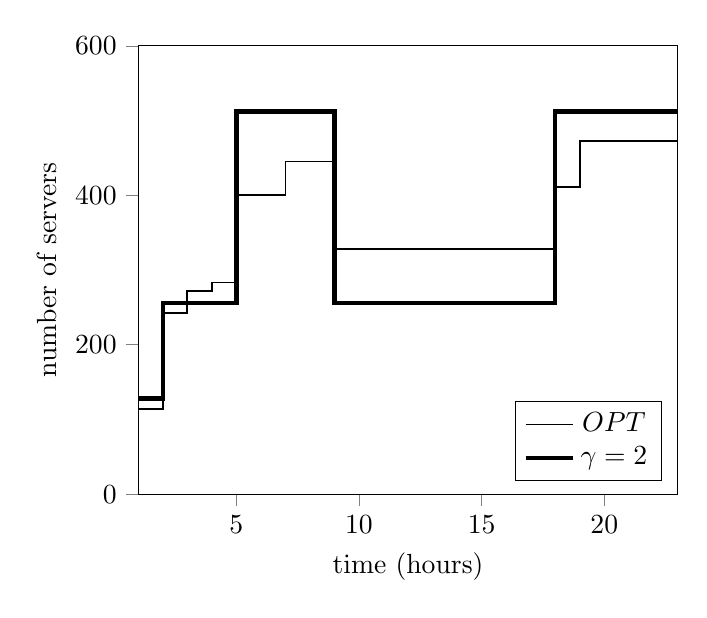
\begin{tikzpicture}

\begin{axis}[
legend pos=south east,
tick align=outside,
tick pos=left,
% x grid style={white!69.0196078431373!black},
xlabel={time (hours)},
xmin=1, xmax=23,
% xtick style={color=black},
% y grid style={white!69.0196078431373!black},
ylabel={number of servers},
ymin=0, ymax=600,
% ytick style={color=black}
]
\addplot [semithick, black, const plot mark left]
table {%
1 114
2 242
3 272
4 283
5 400
6 400
7 445
8 445
9 328
10 328
11 328
12 328
13 328
14 328
15 328
16 328
17 328
18 411
19 473
20 473
21 473
22 473
23 479
};
\addlegendentry{$OPT$}
\addplot [ultra thick, black, const plot mark left]
table {%
1 128
2 256
3 256
4 256
5 512
6 512
7 512
8 512
9 256
10 256
11 256
12 256
13 256
14 256
15 256
16 256
17 256
18 512
19 512
20 512
21 512
22 512
23 512
};
\addlegendentry{$\gamma = 2$}
\end{axis}

\end{tikzpicture}

    \caption{A comparison of the optimal schedule and a schedule found by the approximation algorithm with $\gamma = 2$. The example uses the Facebook 2009-0 trace under our second model. Note that the approximation algorithm is limited to server configurations that are powers of two.}
    \label{fig:a_schedule_found_by_the_multi_dimensional_integral_offline_approximation_algorithm}
\end{figure}

Let $G^{\gamma}$ be the described graph parametrized by $\gamma > 1$. \citeauthor{Albers2021_2}~\cite{Albers2021_2} show that, assuming we are given an instance of SBLO, given a shortest path $P^{\gamma}$ in $G^{\gamma}$, its induced schedule $X^{P^{\gamma}}$ is a $(2\gamma + 1)$-approximation of the optimal schedule $\hat{x}$. Further, the total number of vertices in $G^{\gamma}$ is \begin{align*}
    \mathcal{O}(T |\mathcal{M}|^{\gamma}) = \mathcal{O}(T \prod_{k=1}^d \log_{1+\epsilon} m_k)
\end{align*} as $|M_k^{\gamma}| \in \mathcal{O}(\log_{\gamma} m_k) = \mathcal{O}(\log_{1 + \epsilon} m_k)$. Using the same graph search algorithm that was described in the previous section we are able to find $X^{P^{\gamma}}$ in $\mathcal{O}(T C d \prod_{k=1}^d \log_{1 + \epsilon} m_k)$ time. Hence, setting $\gamma = 1 + \epsilon / 2$ for some $\epsilon > 0$ yields a $(1+\epsilon)$-approximation. The algorithm is described in \cref{alg:md:approximate_graph_search}.

\begin{algorithm}
    \caption{Multi-Dimensional Approximate Graph Search~\cite{Albers2021_2}}\label{alg:md:approximate_graph_search}
    \KwIn{$\mathcal{I}_{\text{Int-SSCO}} = (d \in \mathbb{N}, T \in \mathbb{N}, m \in \mathbb{N}^d, \beta \in \mathbb{R}_{>0}^d, (f_1, \dots, f_T) \in (\mathcal{M} \to \mathbb{R}_{\geq 0})^T)$}
    \For{$t \gets 1$ \KwTo $T$}{
        $(\hat{X}, \hat{c}) \gets \text{\ref{proc:md:optimal_graph_search:handle_first_layer}}(\mathcal{I}_{Int-SSCO}, \mathcal{M}^{\gamma}, \hat{X}, \hat{c}, t, 1, \{\mathbf{0}\})$\;
        $(\hat{X}, \hat{c}) \gets \text{\ref{proc:md:optimal_graph_search:handle_second_layer}}(\mathcal{I}_{Int-SSCO}, \mathcal{M}^{\gamma}, \hat{X}, \hat{c}, t, d, \{(m_1,\dots,m_d)\})$\;
    }
    \Return $\hat{X}^{v_{T,\mathbf{0}}^{\downarrow}}$\;
\end{algorithm}

One important question regarding the approximation algorithm remains. Namely, how to compute the powers of gamma $\gamma^i$ such that $\lfloor\gamma^i\rfloor \in [m_k]$ or $\lceil\gamma^i\rceil \in [m_k]$ for some $k \in [d]$. The simplest solution is to iteratively increase $i \in \mathbb{N}$ until $\gamma^i$ is greater than $\max_{k \in [d]} m_k$. We then keep track of all $\lfloor\gamma^i\rfloor$ and $\lceil\gamma^i\rceil$ that were generated in this way. We observe that this simple approach takes $\mathcal{O}(\log_{\gamma} m_k)$, not altering the runtime of the algorithm. We have thus discussed a polynomial-time approximation scheme for multi-dimensional instances of Int-SSCO.

\begin{figure}
    \begin{subfigure}[b]{.5\linewidth}
    \resizebox{\textwidth}{!}{% This file was created by tikzplotlib v0.9.9.
\begin{tikzpicture}

\begin{axis}[
% tick align=outside,
% tick pos=left,
% x grid style={white!69.0196078431373!black},
xlabel={$\gamma$},
xmin=0.806133272746887, xmax=8.34256508225015,
% xtick style={color=black},
% y grid style={white!69.0196078431373!black},
ylabel={normalized cost},
ymin=0.957275381347888, ymax=1.96641309496129,
% ytick style={color=black}
]
\addplot [mark=x]
table {%
1.14869835499704 1.00314527742122
1.5157165665104 1.03814745510289
2 1.11564992500942
2.63901582154579 1.27894733092918
3.4822022531845 1.46186988151571
4.59479341998814 1.62101371524733
6.06286626604159 1.88422980087979
8 1.92054319888795
};
\end{axis}

\end{tikzpicture}
}
    \caption{Cost}\label{fig:approx_graph_search:cost}
    \end{subfigure}
    \begin{subfigure}[b]{.5\linewidth}
    \resizebox{\textwidth}{!}{% This file was created by tikzplotlib v0.9.9.
\begin{tikzpicture}

\begin{axis}[
% tick align=outside,
% tick pos=left,
% x grid style={white!69.0196078431373!black},
xlabel={$\gamma$},
xmin=0.806133272746887, xmax=8.34256508225015,
% xtick style={color=black},
% y grid style={white!69.0196078431373!black},
ylabel={runtime (seconds)},
ymin=0.17725, ymax=10.35775,
% ytick style={color=black}
]
\addplot [mark=x]
table {%
1.14869835499704 9.895
1.5157165665104 4.410
2 1.518
2.63901582154579 1.975
3.4822022531845 1.823
4.59479341998814 1.450
6.06286626604159 1.115
8 0.640
};
\end{axis}

\end{tikzpicture}
}
    \caption{Runtime}\label{fig:approx_graph_search:runtime}
    \end{subfigure}
    \caption{Normalized cost and runtime of the approximate graph search algorithm for the Facebook 2009-1 trace.}
\end{figure}

In practice, we observe that cost grows linearly with $\gamma$. The normalized cost when used with the Facebook 2009-1 trace is shown in \cref{fig:approx_graph_search:cost}. In contrast, the most significant decrease in runtime occurs for $\gamma \in (1, 2]$ as shown in \cref{fig:approx_graph_search:runtime}.
